% Author: Kailash Ranganathan
% Editor: Dun-Ming Huang, on formatting
% Author Email: kranganathan@berkeley.edu
% CSM16A Spring 2023

\qns{Inverses and Related Topics} \\
% commented out by Damanic Luck since transition to github in fa23 from sp23 doesn't include editnotes in the commonheader.sty
% \editnotes{\\
%     I restructured the answers and some paragraph breaks to make file slightly more readable for SM reviewers. \\
%     I did not change any bold/italicize contents in, so to preserve original intentions of content.

% }

\meta{
    \begin{itemize}
        \item Begin by reviewing invertibility, as well as its conditions. Ensure students gain intuition for why invertibility fails if one of its conditions isn't met (ie. loss of information through nullspaces)
    
        \item Briefly review state transition diagrams, converting the diagrams into transition matrices, and the idea of conservative systems. 
    
        \item The purposes of these questions are to further connect the ideas of state transition matrices and inverses (ie. what does it really \textit{mean} for a state transition matrix to not have an inverse) as well as to hone in on techniques of recognizing invertibility/non-invertibility, such as noticing linear dependence. 
    \end{itemize}
}
% Author: Kailash Ranganathan
% Email: kranganathan@berkeley.edu
% CSM16A Spring 2023
\begin{center}
    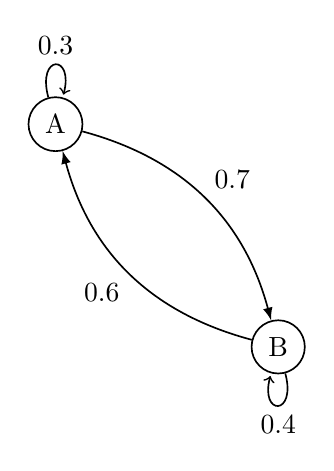
\begin{tikzpicture}[-latex, auto, node distance={4cm}, semithick, main/.style = {draw, circle}]
        \node[main] (A) {A};
        \node[main, below right of = A] (B) {B};
        \path (A) edge[loop above] node{0.3} (A); 
        \path (A) edge[bend left] node{0.7} (B); 
        \path (B) edge[loop below] node{0.4} (B); 
        \path (B) edge[bend left] node{0.6} (A); 
    \end{tikzpicture}
\end{center}

\begin{enumerate}
    \item {
        Say we're given the state transition graph given above. First, write the transition matrix corresponding to the graph. Is it a conservative system?
    }

    \ans{\leavevmode\\
        Say our vector of states is given by 
        \begin{equation*}
                \vec{x}(t) = \begin{bmatrix}
                    a(t) \\
                    b(t) 
                \end{bmatrix} 
        \end{equation*}
        and our transition matrix $\textbf{B}$ satisfies $\vec{x}_{t+1} = \textbf{B} \vec{x}_t$. \leavevmode \\
        Then, by noting edge weights on the graph from the previous page, we can see that $\boxed{\textbf{B} = \begin{bmatrix}
            0.3 & 0.6 \\
            0.7 & 0.4 
        \end{bmatrix}}$. \leavevmode \\
        Each column sums to one in the matrix, so the system $\boxed{\textbf{is conservative.}}$. If we interpret the values $a(t)$ and $b(t)$ as some sort of material, this means the total material in the system is constant over time -- no loss/gain.
    }

    \item {
        Now suppose that we're given a different state transition graph with the transition matrix $\textbf{T}$ given by
            \begin{equation*}
            \textbf{T} = \begin{bmatrix}
                0.2 & 0.4 & 0.1 \\
                0.4 & 0.8 & 0.1 \\
                0.6 & 1.2 & 0.3 \\
            \end{bmatrix}
            \end{equation*}
        \textbf{Show that the matrix is \textit{not} invertible} \\
        (you could do this the "long way" or do less work by noticing something about the columns). 
    }

    \ans{ \leavevmode \\
        Here, one option is to do Gaussian elimination on the matrix and realize that there are not pivots in every column. But frankly, that'd be a bit involved and error-prone, especially with a 3x3 matrix and one with decimal values too. \leavevmode \\
        The first thing you should \textit{always} do before Gaussian eliminating is glance at the columns for clear signs of dependence. After looking, we can see that the second column of \textbf{T} is twice that of the first. \leavevmode \\
        That is, $2\begin{bmatrix}
            0.2 \\
            0.4 \\
            0.6
        \end{bmatrix} = \begin{bmatrix}
            0.4 \\
            0.8 \\
            1.2
        \end{bmatrix}$. \leavevmode\\
        Thus, the columns must be linearly dependent, because we could do a non-zero linear combination of them, set the third column to zero and the first column to negative twice of the second column, and always arrive at zero. \\
        Linearly dependent columns imply a non-full-rank matrix and non-trivial nullspace, all indications that the matrix is \boxed{\textbf{not invertible}}. 
    }

    \item {
        For state transition matrices, the above result implies that if we're in some state $\vec{y}$ at time $t$, we \textit{cannot} recover a unique state $\vec{x}$ at time $t-1$ that we came from. \\
        We want to further understand this claim -- given some $\vec{x}$ and $\vec{y}$ such that $\vec{y} = \textbf{T} \vec{x}$, demonstrate that the $\vec{x}$ is non-unique by finding the set of all valid solutions to $\vec{y} = \textbf{T} \vec{x}$ for the above matrix given that $\vec{x}$ is a valid solution.
        \par
        \emph{Hint: Think of the conditions of invertibility (and thus, what is violated in the case of non-invertibility)? Which one of these relate to the uniqueness/existence of solutions to matrix equations? }
    }
    \ans{
        There are two key insights to answering this question. \\
        The first one is to recognize that a non-invertible matrix must have a non-trivial/non-zero nullspace, and the second one is to realize that a non-zero nullspace implies the lack of uniqueness for solutions to the linear system given by the matrix. \\
        The first insight is just gathered by knowledge of invertibility, but I'll briefly describe how the second step leads us to our answer.
        \par
        Given a linear system $\vec{y} = \textbf{T} \vec{x}$, suppose we thought $\vec{x}$ was a unique solution but the matrix had a non-zero nullspace. Then, for some vector $\vec{u}$ in the nullspace of \textbf{T} implying $\textbf{T} \vec{u} = 0$, we could do the following: 
        \begin{equation}
        \vec{y} = \textbf{T} \vec{x} = \textbf{T} \vec{x} + 0 = \textbf{T} \vec{x} + \textbf{T} \vec{u} = \textbf{T} (\vec{x} + \vec{u})
        \end{equation}
        but then $\vec{x} + \vec{u}$ is also a solution to the equation, so $\vec{x}$ can't be a unique solution. This is a key point -- any matrix with a nontrivial nullspace \textit{cannot} have unique solutions, else we could just add any nullspace vector, and as its output would be $0$ by definition, it would not change the output of the system at all! \\
        Going back to our question, if $\vec{x}$ is a solution, then $\vec{x}$ plus any nullspace vector of \textbf{T} is also a solution. So, this question comes down to finding the nullspace of \textbf{T}. \\
        Remember from the previous question that twice the first column times negative of the second column plus zero times the last column equals zero to prove linear dependence. \\
        We can extend this to a nullspace vector, where any vector satisfying $\alpha \begin{bmatrix}
            2 \\
            -1 \\
            0 \\
        \end{bmatrix}, \alpha \in \mathbb{R}$ will be in the nullspace. \\
        Hence, the total set of solutions satisfy $\vec{x} + \alpha \begin{bmatrix}
            2 \\
            -1 \\
            0 \\
        \end{bmatrix}, \alpha \in \mathbb{R} = \boxed{\vec{x} + \textbf{span} \left \{\begin{bmatrix}
            2 \\
            -1 \\
            0 \\
        \end{bmatrix} \right \}} $.
        \par
        (Note, you can definitely also do this question using Gaussian elimination to find the nullspace too -- this just illustrates a quicker method). 
    }

    \item {
        What the previous part tells us about state transition matrices is pretty interesting. If we have a graph such that its transition matrix is invertible, we cannot know what unique state we came from at any point in time! Say your classmate claims that any conservative system \textit{must} have an inverse and thus must be reversible in time. Prove (or disprove) this statement. \emph{Hint: Just one valid counter-example can disprove the claim entirely.}
    }

    \ans{ \leavevmode\\
        The limitation of conservative systems just means that columns have to sum to one. But we could have two columns be the exact same and still be conservative. In fact, we could have every column be the same and still be conservative if they sum to one. \leavevmode \\
        Thus, it's clear from this line of reasoning to come up with counter examples which are definitely not invertible due to lack of linear dependence. One example is $\begin{bmatrix}
            1/3 & 1/3 & 1/3 \\
            1/3 & 1/3 & 1/3 \\
            1/3 & 1/3 & 1/3 
        \end{bmatrix}$, which as you can verify, is definitely conservative and definitely non-invertible.
    }

    \item {
        Lets take the matrix 
        \begin{equation}
            \textbf{A} = \begin{bmatrix}
                0 & a & b \\
                c & 0 & d \\
                e & f & 0 \\
            \end{bmatrix}
        \end{equation}
        If you draw the graph represented by this matrix, you should get a perfectly cyclical graph! Given the condition $abcdef \neq = 0$, show that the matrix is not necessarily invertible. \emph{Hint: Remember, just one counterexample is a valid "disproof"!}
    }

    \ans{\leavevmode \\
        Here, at least, we know that we are looking for linear dependence because the question states the matrix is not necessarily invertible. Think of what linear dependence means -- columns such that they have a non-zero combination summing to zero (and we know any of the variables can't be zero). \leavevmode \\
        As a start, set one of the variables, say $a$, to some value, say $1$. Immediately, we see $b$ must cancel that out for linear dependence, so $b = -1$. Then, we can notice all the variables come in pairs -- each variable must be a negative of its pair for linear dependence, but this is perfectly doable with the condition $abcdef \neq 0$, just set $a = -b$, $c = -d$, and $e = -f$. \leavevmode \\
        Thus, one sample matrix that satisfies the constraints and is non-invertible (by linear dependence of columns) is $\begin{bmatrix}
            0 & 1 & -1 \\
            1 & 0 & -1 \\
            1 & -1 & 0 
        \end{bmatrix}$, but anything such that the row-wise pairs are negatives works. 
    }

    \item{
        Lastly, lets take the exact same problem as \textbf{(e)}, except now we assert that exactly \textit{one} of $a, b, c, d, e, f$ is zero. Show that the matrix $\textbf{A}$ \textit{must} be invertible. \emph{Hint: Try setting different variables to zero, and see if you can somehow arrive at impossibility of linear dependence. What does that tell you?}
    }

    \ans{
        Interestingly, this small change of condition can change the entire property of invertibility for the matrix. \\
        Here, notice that rather than looking for linear dependence, we're looking for a guarantee of linear independence of columns, as the matrix $\textit{must}$ be invertible. \\
        Once again, lets start with the condition and explore. Suppose we set $a = 0$. If we try to construct a non-invertible matrix, $b$ would have to be $0$ as well, else there's no non-zero coefficient we could multiply it by to get the first component of the linear combination of columns to be zero (this is true because $a$ and $b$ are the only potentially non-zero terms on the first row, and to get 0 by a linear combination, every row sum needs to be 0). \\
        Think about this idea for a bit, and eventually it shows that this is true for all pairs of variables. If $a = 0$, then $b = 0$ for linear dependence -- similarly for $c = 0$ then $d = 0$, and if $e = 0$ then $f = 0$. \\
        However, none of these are possible because only exactly one variable can be zero, so there's no way to get linear dependence/columns combining to zero with this constraint. Thus, the matrix \textit{must} be invertible due to having linearly independent columns.     
    }
    
    % \notes{\\
    %     The last couple examples may seem quite contrived, but in general, it's very useful to understand the tight relationship between invertibility and linear independence/dependence of columns, as well as tricks/intuition for how to recognize linear dependence/independence in matrices when pure Gaussian elimination may not work. It's also useful to be able to very rigorously define the assumptions/conditions under which properties such as invertibility hold -- for example, it might be tempting to say conservative systems must be invertible as they "conserve" quantity from one state to another, but as we showed, this isn't necessarily true. Counterexamples FTW! 
    % }
    
\end{enumerate}